\documentclass[a4paper,10.5pt]{article}

%%%%%%%%%%%%%%%%%%%%%%%%%%%%%%%%%%%%%%%%%%%%%%%%%%%%%%
%%                 PACKAGES
%%%%%%%%%%%%%%%%%%%%%%%%%%%%%%%%%%%%%%%%%%%%%%%%%%%%%%
\usepackage[T1]{fontenc}
\usepackage[utf8]{inputenc}
\usepackage[a4paper, top=2.6cm, bottom=2.2cm, left=1.6cm, right=1.6cm, headheight=26pt, headsep=14pt, footskip=32pt]{geometry}
\usepackage{amsmath,amssymb}
\usepackage{graphicx}
\usepackage{booktabs}
\usepackage{array}
\usepackage{tikz}
\usepackage{xcolor}
\usepackage{multicol}
\usepackage{titlesec}
\usepackage{enumitem}
\usepackage{fancyhdr}
\usepackage{lastpage}
\usepackage{hyperref}
\usetikzlibrary{positioning, calc, arrows.meta}

%%%%%%%%%%%%%%%%%%%%%%%%%%%%%%%%%%%%%%%%%%%%%%%%%%%%%%
%%                 COLORS (IDENTITE ASR)
%%%%%%%%%%%%%%%%%%%%%%%%%%%%%%%%%%%%%%%%%%%%%%%%%%%%%%
\definecolor{bgBase}{RGB}{252,252,254}
\definecolor{bgBlock}{RGB}{242,245,250}
\definecolor{primary}{RGB}{10,37,64}
\definecolor{accent}{RGB}{0,195,255}
\definecolor{accentSoft}{RGB}{210,247,255}
\definecolor{good}{RGB}{0,168,120}
\definecolor{text}{RGB}{40,45,55}
\definecolor{muted}{RGB}{140,150,165}
\definecolor{alertRed}{RGB}{214,40,40}

\pagecolor{bgBase}
\color{text}

%%%%%%%%%%%%%%%%%%%%%%%%%%%%%%%%%%%%%%%%%%%%%%%%%%%%%%
%%                 METADONNEES DU DOCUMENT
%%%%%%%%%%%%%%%%%%%%%%%%%%%%%%%%%%%%%%%%%%%%%%%%%%%%%%
\newcommand{\paperTitle}{The 1900 Thesis That Invented Quant Finance}
\newcommand{\paperSubtitle}{Louis Bachelier and the Origins of the Random Walk}
\newcommand{\paperNote}{Thursday Deepthink No.~01}
\newcommand{\paperLogo}{assets/logo/logo.png}

%%%%%%%%%%%%%%%%%%%%%%%%%%%%%%%%%%%%%%%%%%%%%%%%%%%%%%
%%       LOGO ROBUSTE (repli si fichier absent)
%%%%%%%%%%%%%%%%%%%%%%%%%%%%%%%%%%%%%%%%%%%%%%%%%%%%%%
\newcommand{\roundlogo}[2][1.9cm]{%
    \IfFileExists{#2}{%
        \begin{tikzpicture}
            \node[rectangle, rounded corners=0.28cm, minimum width=#1, minimum height=#1,
                  path picture={
                      \node at (path picture bounding box.center) {
                          \includegraphics[width=#1, keepaspectratio]{#2}
                      };
                  }] {};
        \end{tikzpicture}%
    }{%
        \begin{tikzpicture}
            \node[rectangle, rounded corners=0.28cm, minimum width=#1, minimum height=#1,
                  fill=primary] (box) {};
            \node[white, font=\bfseries\normalsize] at (box.center) {ASR};
        \end{tikzpicture}%
    }%
}
% Version miniature pour l'en-tête courant (pages 2+)
\newcommand{\minilogo}[1]{%
    \IfFileExists{#1}{%
        \begin{tikzpicture}
            \node[rectangle, rounded corners=0.09cm, minimum width=0.55cm, minimum height=0.55cm,
                  path picture={
                      \node at (path picture bounding box.center) {
                          \includegraphics[width=0.55cm, keepaspectratio]{#1}
                      };
                  }] {};
        \end{tikzpicture}%
    }{%
        
\begin{tikzpicture}
            \node[rectangle, rounded corners=0.09cm, minimum width=0.55cm, minimum height=0.55cm,
                  fill=primary] (box) {};
            \node[white, font=\bfseries\tiny] at (box.center) {ASR};
        \end{tikzpicture}%
    }%
}

%%%%%%%%%%%%%%%%%%%%%%%%%%%%%%%%%%%%%%%%%%%%%%%%%%%%%%
%%       EN-TETE / PIED DE PAGE COURANTS (pages 2+)
%%%%%%%%%%%%%%%%%%%%%%%%%%%%%%%%%%%%%%%%%%%%%%%%%%%%%%
\pagestyle{fancy}
\fancyhf{}
\renewcommand{\headrulewidth}{1pt}
\renewcommand{\footrulewidth}{0.7pt}
\renewcommand{\headrule}{{\color{accent}\hrule height\headrulewidth}}
\renewcommand{\footrule}{{\color{accent}\hrule height\footrulewidth}}

\fancyhead[L]{%
    \raisebox{-0.12cm}{\minilogo{\paperLogo}}\hspace{6pt}%
    {\small\bfseries\color{primary}\paperTitle}%
    \;{\small\color{muted}\textbar\; \paperSubtitle}%
}
\fancyhead[R]{\small\color{muted}\paperNote}
\fancyfoot[L]{\footnotesize\color{muted}\textbf{Alpha Stochastic Research}}
\fancyfoot[C]{\footnotesize\color{muted}
  \href{mailto:contact@asr-lab.online}{contact@asr-lab.online}}
\fancyfoot[R]{\footnotesize\color{muted}Page \thepage\ / \pageref{LastPage}}

% Style de la 1ere page : pas d'en-tête courant
\fancypagestyle{firstpage}{%
  \fancyhf{}
  \fancyfoot[L]{\footnotesize\color{muted}\textbf{Alpha Stochastic Research}}
  \fancyfoot[C]{\footnotesize\color{muted}
    \href{mailto:contact@asr-lab.online}{contact@asr-lab.online}}
  \fancyfoot[R]{\footnotesize\color{muted}Page \thepage\ / \pageref{LastPage}}
  \renewcommand{\headrulewidth}{0pt}
  \renewcommand{\footrulewidth}{0.7pt}
  \renewcommand{\footrule}{{\color{accent}\hrule height\footrulewidth}}
}

%%%%%%%%%%%%%%%%%%%%%%%%%%%%%%%%%%%%%%%%%%%%%%%%%%%%%%
%%                 TITRES DE SECTION
%%%%%%%%%%%%%%%%%%%%%%%%%%%%%%%%%%%%%%%%%%%%%%%%%%%%%%
\titleformat{\section}
  {\normalfont\Large\bfseries\color{primary}}
  {}{0em}{}
  [{\color{accent}\titlerule[1.4pt]}]
\titlespacing*{\section}{0pt}{12pt}{6pt}

\titleformat{\subsection}
  {\normalfont\normalsize\bfseries\color{primary}}
  {}{0em}{}
\titlespacing*{\subsection}{0pt}{8pt}{3pt}

\setlength{\columnsep}{22pt}
\setlength{\parindent}{0pt}
\setlength{\parskip}{4pt}

\hypersetup{colorlinks=true, urlcolor=accent, linkcolor=accent}

\begin{document}

%%%%%%%%%%%%%%%%%%%%%%%%%%%%%%%%%%%%%%%%%%%%%%%%%%%%%%
%%       MASTHEAD (page 1 uniquement)
%%%%%%%%%%%%%%%%%%%%%%%%%%%%%%%%%%%%%%%%%%%%%%%%%%%%%%
\thispagestyle{firstpage}

\begin{minipage}[c]{0.13\linewidth}
    \roundlogo[2cm]{\paperLogo}
\end{minipage}%
\begin{minipage}[c]{0.87\linewidth}
    \raggedright
    {\fontsize{27}{31}\selectfont\bfseries\color{primary} \paperTitle\par}
    \vspace{3pt}
    {\Large\color{accent}\bfseries \paperSubtitle\par}
\end{minipage}

\vspace{6pt}
{\color{accent}\rule{\linewidth}{1.3pt}}
\vspace{4pt}

\noindent{\small\color{muted}
\textbf{Alpha Stochastic Research} \quad$\cdot$\quad Stochastic Research \& Open Science
\hfill
\today \quad$\cdot$\quad \paperNote
\par}

\vspace{10pt}

\noindent\colorbox{bgBlock}{%
  \begin{minipage}{\dimexpr\linewidth-16pt\relax}
    \vspace{5pt}
    \textbf{\color{primary}Abstract.}\;\small
    Five years before Albert Einstein published his famous paper on Brownian motion, a French mathematician named Louis Bachelier modeled the stock market using the exact same mathematics. Bachelier's 1900 thesis, \textit{Théorie de la Spéculation}, was the very first time advanced probability theory was applied to financial markets. He single-handedly birthed the concept of the ``random walk'' and laid the absolute groundwork for quantitative finance, 70 years before Black and Scholes.
    \vspace{5pt}
  \end{minipage}%
}

\vspace{12pt}

%%%%%%%%%%%%%%%%%%%%%%%%%%%%%%%%%%%%%%%%%%%%%%%%%%%%%%
%%       CORPS DE L'ARTICLE
%%%%%%%%%%%%%%%%%%%%%%%%%%%%%%%%%%%%%%%%%%%%%%%%%%%%%%
\begin{multicols}{2}
\small

\section*{1. The Core Ideas}

\subsection*{1.1 The Martingale Concept}
Bachelier famously stated that \textit{``the mathematical expectation of the speculator is zero.''} This profound insight implies that the market is inherently fair and unpredictable. In modern terms, he identified that asset prices follow a \textbf{Martingale} process, where the current price is the best predictor of the future price.

\subsection*{1.2 The Random Walk}
He argued mathematically that past price movements contain absolutely no information about future price movements. This laid the structural foundation for the \textbf{Efficient Market Hypothesis (EMH)}, developed decades later by Eugene Fama.

\section*{2. The Mathematics Behind It}
Bachelier modeled asset prices using what we now call \textbf{Arithmetic Brownian Motion}. He established that price changes follow a normal distribution, driven by the heat equation (diffusion equation):
$$
\frac{\partial P}{\partial t} = \frac{1}{2} k \frac{\partial^2 P}{\partial x^2}
$$
Meaning the probability of a price change spreads out over time exactly like heat diffusing through a piece of metal. 

\vspace{5pt}
Furthermore, he developed the very first analytical formula to value options, recognizing a fundamental principle of quantitative finance: \textbf{volatility scales with the square root of time} ($\sqrt{t}$).

\begin{center}
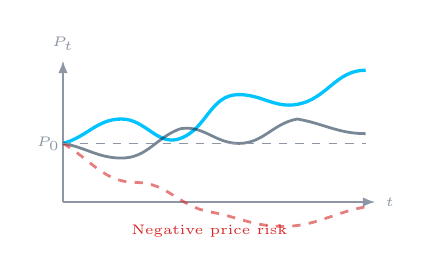
\begin{tikzpicture}[scale=0.62]
    \draw[muted, thick, -{Latex[length=1.6mm]}] (0,0) -- (6.4,0) node[right, font=\tiny, color=muted] {$t$};
    \draw[muted, thick, -{Latex[length=1.6mm]}] (0,0) -- (0,2.9) node[above, font=\tiny, color=muted] {$P_t$};
    \draw[accent, line width=1.2pt]
        (0,1.2) to[out=15,in=180] (1.2,1.7) to[out=0,in=200] (2.4,1.3)
        to[out=20,in=180] (3.6,2.2) to[out=0,in=190] (4.8,2.0) to[out=10,in=180] (6.2,2.7);
    \draw[primary, opacity=0.55, line width=1pt]
        (0,1.2) to[out=-10,in=180] (1.2,0.9) to[out=0,in=200] (2.4,1.5)
        to[out=10,in=180] (3.6,1.2) to[out=0,in=190] (4.8,1.7) to[out=-10,in=180] (6.2,1.4);
    \draw[alertRed, opacity=0.6, line width=1pt, dashed]
        (0,1.2) to[out=-30,in=180] (1.5,0.4) to[out=0,in=170] (3.0,-0.2) 
        to[out=-10,in=180] (4.5,-0.5) to[out=0,in=190] (6.2,-0.1); % Illustrates negative prices
    \draw[muted, dashed] (0,1.2) -- (6.2,1.2);
    \node[font=\tiny, color=muted] at (-0.3, 1.2) {$P_0$};
    \node[font=\tiny, color=alertRed] at (3.0, -0.6) {Negative price risk};
\end{tikzpicture}
\end{center}
\centerline{\tiny\color{muted} Fig. 1 — Arithmetic Random Walk Paths}

\section*{3. Limitations of the Model}
Bachelier used an \textit{arithmetic} random walk rather than a geometric one. This implies that price changes are normally distributed, which theoretically allows stock prices to drop below zero (as illustrated by the red dashed line in Fig. 1). 

Furthermore, the model assumes constant volatility and ignores the ``fat tails'' (extreme market events) we see in real financial data. It was Paul Samuelson in 1965 who fixed the negative price issue by introducing \textbf{Geometric Brownian Motion}, replacing standard normal distribution with log-normal distribution.

\section*{4. Applications Today}
While his specific formula isn't used directly to trade today, his framework is the DNA of modern finance. It paved the way for:
\begin{itemize}[leftmargin=12pt, itemsep=2pt, topsep=3pt]
    \item[\textcolor{accent}{$\blacksquare$}] Itô Calculus and Stochastic Differential Equations.
    \item[\textcolor{accent}{$\blacksquare$}] The Efficient Market Hypothesis.
    \item[\textcolor{accent}{$\blacksquare$}] The Black-Scholes-Merton option pricing model.
\end{itemize}

\section*{5. Conclusion}
Bachelier's genius was largely ignored during his lifetime. The mathematical community viewed his work on finance as ``unworthy'' of pure mathematics. Yet today, his thesis stands as a testament to the power of cross-disciplinary thinking, proving that the chaotic movement of human crowds trading assets can be described by the very same laws governing thermodynamics.

\section*{References}
\footnotesize
Bachelier, L. (1900). \emph{Théorie de la spéculation}. Annales Scientifiques de l'École Normale Supérieure, 17, 21-86.\\[4pt]
Cootner, P. H. (1964). \emph{The Random Character of Stock Market Prices}. MIT Press.\\[4pt]
Samuelson, P. A. (1965). \emph{Rational Theory of Warrant Pricing}. Industrial Management Review, 6(2), 13-31.

\end{multicols}

\end{document}
